\chapter{System Design and Methodology}
\label{ch:design}

\section{System Overview}

The system is organized into four modules built on a shared data foundation
(Figure~\ref{tab:pipeline}). \textbf{Module~A} classifies donation
\emph{intent} at the whole-dialogue level. \textbf{Module~B} -- the deepest
and most extensively iterated part of this project -- recognizes persuasion
\emph{strategies} at the turn level, multi-label, at two granularities (41
strategies / 11 categories). \textbf{Module~C} uses Module~B's gold labels to
model donation \emph{outcome}. \textbf{Module~D} re-applies Module~A's
architecture to a second, generic persuasive domain to test transfer. All
four modules share the annotated corpus described in
Section~\ref{sec:annotation}.

\begin{table}[H]
\centering
\caption{End-to-end pipeline, module by module.}
\label{tab:pipeline}
\begin{tabular}{@{}p{2.1cm}p{4.6cm}p{4.6cm}p{2.7cm}@{}}
\toprule
\textbf{Stage} & \textbf{Input} & \textbf{Output} & \textbf{Module} \\
\midrule
1. Annotation & Raw P4G dialogues (persuader turns) & 41-strategy / 11-category multi-label per turn & Data (\S\ref{sec:annotation}) \\
2. Split & Annotated turns & Dialogue-grouped 70/15/15 train/val/test & Data (\S\ref{sec:split}) \\
3. Strategy recognition & Turn text + 5-turn context & Per-label probabilities $\to$ decision sets & B (\S\ref{sec:design-module-b}) \\
4. Outcome model & Gold strategy sets (dialogue-level) & Strategy $\to$ donation association & C (\S\ref{sec:design-module-c}) \\
5. Intent classification & Full dialogue transcript & Binary intent + modifier & A (\S\ref{sec:design-module-a}) \\
6. Domain transfer & Buyer--seller dialogues & Same intent architecture, new domain & D (\S\ref{sec:design-module-d}) \\
\bottomrule
\end{tabular}
\end{table}

\section{Dataset and Annotation}
\label{sec:annotation}

\subsection{Taxonomy}
\label{sec:taxonomy}

The taxonomy was designed to be exhaustive over the tactics observed in a
sample of P4G dialogues while staying small enough to annotate and model
tractably. It has 11 categories and 41 strategies (Table~\ref{tab:taxonomy}),
each category holding 3--4 strategies. Each strategy carries a short
definition and a small set of example cue phrases used to anchor annotator
judgment (and, later, reused as zero-shot cue features for the classifier,
Section~\ref{sec:design-ensemble}).

\begin{table}[H]
\centering
\caption{The 11-category / 41-strategy taxonomy (strategy counts per category).}
\label{tab:taxonomy}
\begin{tabular}{@{}lc@{}}
\toprule
\textbf{Category} & \textbf{\# Strategies} \\
\midrule
Rational Appeal & 4 \\
Emotional Appeal & 4 \\
Credibility Appeal & 4 \\
Social Influence & 4 \\
Reciprocity and Exchange & 3 \\
Commitment and Consistency & 4 \\
Framing and Presentation & 4 \\
Urgency and Scarcity & 3 \\
Threat and Pressure & 3 \\
Information Provision & 4 \\
Relational and Interactive & 4 \\
\midrule
\textbf{Total} & \textbf{41} \\
\bottomrule
\end{tabular}
\end{table}

\subsection{Annotation Process}

Annotation was applied to the first 10{,}600 persuader turns of the corpus
(1{,}017 dialogues), in five contiguous segments produced independently and
concatenated in the corpus's own row order (Table~\ref{tab:annotation-segments}).
Each turn was labeled using its own text plus the five immediately preceding
dialogue turns (alternating persuader/persuadee) as context, since several
strategies -- e.g. a direct answer to a persuadee's question -- cannot be
correctly identified from the turn text alone.

\begin{table}[H]
\centering
\caption{Annotation segments, in canonical corpus row order.}
\label{tab:annotation-segments}
\begin{tabular}{@{}clr@{}}
\toprule
\textbf{Turn range} & \textbf{Annotator} & \textbf{Turns} \\
\midrule
1 -- 2{,}000 & Segment 1 & 2{,}000 \\
2{,}001 -- 4{,}000 & Segment 2 & 2{,}000 \\
4{,}001 -- 6{,}000 & Segment 3 (model-batch run) & 2{,}000 \\
6{,}001 -- 7{,}000 & Segment 2 (continued) & 1{,}000 \\
7{,}001 -- 10{,}600 & Segment 4 & 3{,}600 \\
\midrule
\textbf{Total} & & \textbf{10{,}600} \\
\bottomrule
\end{tabular}
\end{table}

Labeling was carried out by an LLM agent (Claude) working directly from the
taxonomy definitions, cue phrases, and decision rules, under a documented
\textbf{human verification checkpoint}: annotation stopped after an initial
batch for manual review against the guideline before the remainder of a
segment was processed, and batches were regenerated and re-reviewed where the
checkpoint surfaced systematic disagreement with the intended taxonomy
semantics. This is disclosed here in full because it directly affects how
the classifier's results should be read: Section~\ref{sec:ceiling} measures
the reliability of \emph{this specific} annotation process (rather than
assuming human-level reliability by default) and reports classifier
performance against that measured ceiling.

\subsection{Split}
\label{sec:split}

The corpus is split 70/15/15 into train/validation/test using a
dialogue-\emph{grouped} stratified split (\texttt{MultilabelStratifiedKFold},
7 folds, fixed seed), so that no dialogue's turns appear in more than one
split -- turns from the same dialogue share style and context and would leak
information across a turn-level split. This yields 7{,}592 training, 1{,}513
validation, and 1{,}495 test turns. Every downstream cross-validated
procedure in this report (decision-threshold fitting, bootstrap resampling,
significance testing) resamples by dialogue for the same reason.

\subsection{Exploratory Statistics}
\label{sec:eda}

Table~\ref{tab:eda} summarizes the annotated corpus. The mean of 1.68
strategies (1.50 categories) per turn, with fewer than 7\% of turns carrying
no label at all, confirms that a single-label formulation would misrepresent
the data: a persuader turn routinely does more than one persuasive thing at
once. Label prevalence is heavily right-skewed at the strategy level (the
most common strategy, \textit{rapport\_building}, occurs 2{,}860 times; the
rarest, \textit{door\_in\_the\_face}, occurs twice) -- an imbalance ratio of
roughly 1{,}430$\times$ -- but far more moderate at the category level
(\textit{Relational and Interactive} at 46.2\% down to \textit{Urgency and
Scarcity} at 1.5\%, a ratio of roughly 30$\times$). This gap between the two
granularities' imbalance is the empirical basis for the category-first
reframing described in Section~\ref{sec:category-first}.

\begin{table}[H]
\centering
\caption{Corpus statistics (all 10{,}600 annotated turns).}
\label{tab:eda}
\begin{tabular}{@{}lr@{}}
\toprule
Turns / Dialogues & 10{,}600 / 1{,}017 \\
Mean turns per dialogue & 10.42 (range 4--15) \\
Mean strategy-labels per turn & 1.679 \\
Mean category-labels per turn & 1.504 \\
Turns with zero labels & 707 (6.7\%) \\
Turns with $\geq$2 labels & 48.9\% \\
Strategy imbalance ratio (max/min prevalence) & $\approx$1{,}430$\times$ \\
Category imbalance ratio (max/min prevalence) & $\approx$30$\times$ \\
\bottomrule
\end{tabular}
\end{table}

\begin{figure}[H]
\centering
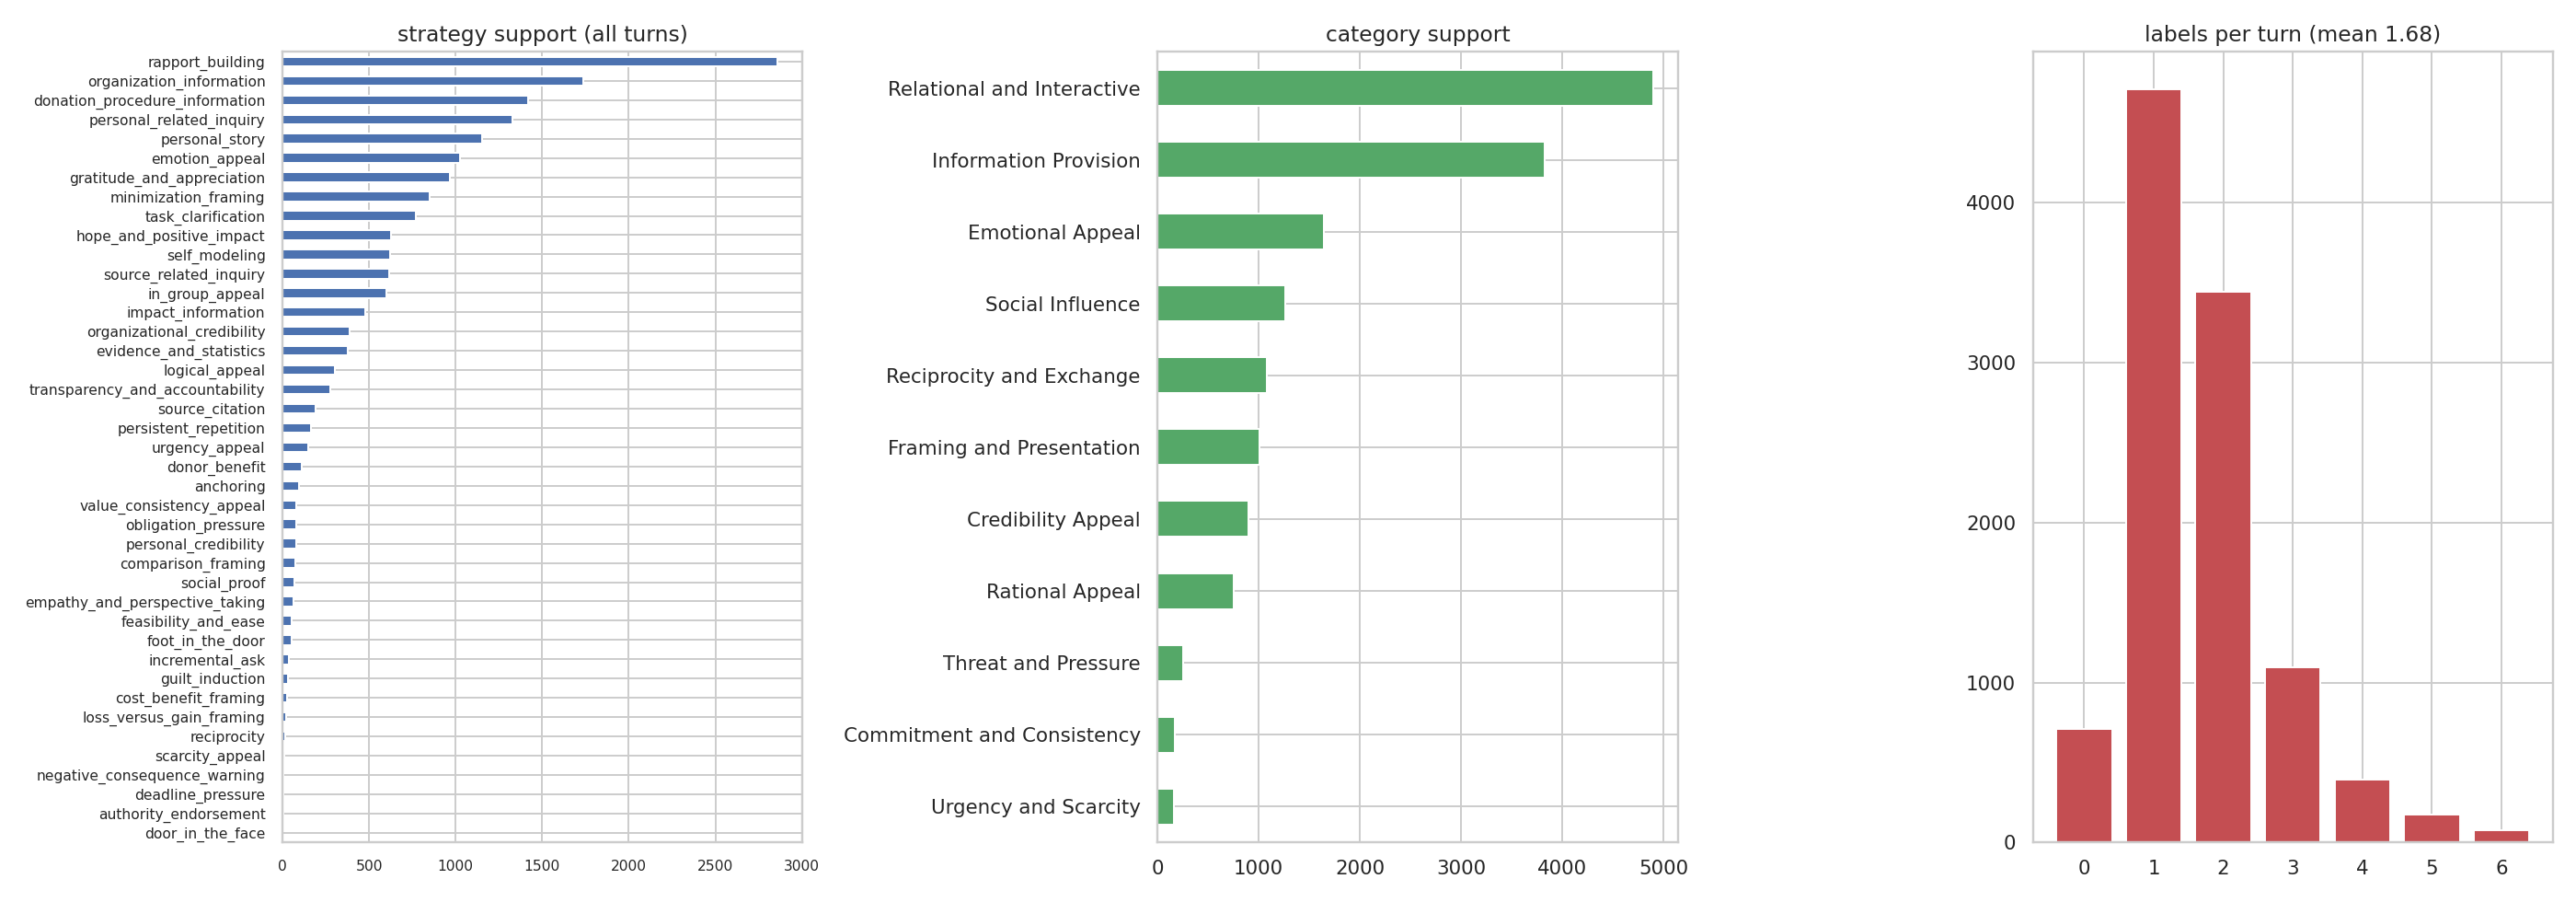
\includegraphics[width=0.85\textwidth]{figures/fig_label_distribution.png}
\caption{Strategy and category label-prevalence distribution across the annotated corpus.}
\label{fig:label-dist}
\end{figure}

\section{Module A: Donation-Intent Classification}
\label{sec:design-module-a}

Module~A classifies a complete dialogue's donation intent (binary: intent
present or absent) and, when present, its modifier (outright, deferred, or
conditional). Its final architecture -- referred to in project records as
\emph{Antiphony} (v14) -- encodes the persuader's and persuadee's turns as
two role-pure streams, applies directional cross-attention between the two
streams so that each side's representation is conditioned on the other's
history, and tracks the dialogue's evolving state with a trajectory
recurrent unit before a final classification head. This architecture was
reached after thirteen prior iterations spanning flat sequence baselines,
speaker-aware encoding, hierarchical dialogue encoders, and specialist
routing, each evaluated on held-out data before being superseded (results in
Section~\ref{sec:module-a-results}).

\section{Module B: Multi-Label Persuasion-Strategy Classifier}
\label{sec:design-module-b}

\subsection{Encoder Architecture}

Each ensemble member is a single pretrained transformer encoder with a
speaker-role embedding added to its token representations (marking whether
each token belongs to a persuader or persuadee turn, resolved from the
literal \texttt{[Persuader]}/\texttt{[Persuadee]} markers already present in
the input text via the tokenizer's character-offset mapping), an
attention-pooling layer over the resulting sequence (measured to consistently
outperform mean pooling), multi-sample dropout before the classification
heads for a cheap ensembling-within-a-model effect, and \emph{two} linear
heads sharing the pooled representation: a 41-way strategy head and an
11-way category head. Table~\ref{tab:members-v17} lists the seven encoder
members used in the final iteration.

\begin{table}[H]
\centering
\caption{Encoder ensemble members, final iteration (v17). ``Orientation'' marks a member as
tuned for the micro or macro objective (Section~\ref{sec:objective-split}).}
\label{tab:members-v17}
\begin{tabular}{@{}lccc@{}}
\toprule
\textbf{Member} & \textbf{Backbone} & \textbf{Context} & \textbf{Orientation} \\
\midrule
\texttt{robertaL-ctx0} & RoBERTa-large & 0 turns & micro \\
\texttt{roberta-ctx0} & RoBERTa-base & 0 turns & micro \\
\texttt{electra-ctx0} & ELECTRA-base & 0 turns & micro \\
\texttt{roberta-ctx0-s7} & RoBERTa-base & 0 turns & macro \\
\texttt{roberta-ctx3-mac} & RoBERTa-base & 3 turns & macro \\
\texttt{robertaL-ctx0-mac} & RoBERTa-large & 0 turns & macro \\
\texttt{roberta-ctx0-mac} & RoBERTa-base & 0 turns & macro \\
\bottomrule
\end{tabular}
\end{table}

\subsection{Loss Function}
\label{sec:design-loss}

Each head is trained with Asymmetric Loss \citep{benbaruch2021asl}, which
applies a stronger focusing exponent to easy negatives than to positives and
subtracts a small probability margin from the negative branch before the
log term, so that a label the model is already confidently (and correctly)
predicting absent contributes almost nothing to the gradient -- important
here because with 41 labels the overwhelming majority of (turn, label)
pairs are true negatives. \emph{Micro}-oriented members additionally apply
Distribution-Balanced rebalancing \citep{wu2020distribution}, and
\emph{macro}-oriented members apply a per-label positive-class weight
(capped to avoid destabilizing training on the rarest labels); the choice of
which members get which treatment is itself an empirical finding, not a
default, and is documented in Section~\ref{sec:objective-split}.

\subsection{Data Augmentation}
\label{sec:design-augmentation}

Turns carrying a rare strategy are duplicated with light EDA-style
perturbation (synonym replacement and word swap, confined to the turn being
labeled so the dialogue context is never corrupted) to give the encoder more
gradient signal on the rare tail. This was measured to help some
configurations and hurt others (Section~\ref{sec:ablation-augmentation}), and
in the final design is applied only to micro-oriented members.

\subsection{Ensemble and Decoding}
\label{sec:design-ensemble}

Seven fine-tuned encoders, seven corresponding few-shot nearest-centroid
prototype members (a lightweight alternative that scores a turn by cosine
similarity to the centroid of each label's training-turn embeddings, useful
as a diversity source for the ensemble search), two shallow TF-IDF
classifiers (logistic regression and gradient-boosted trees), and two
zero-shot ``cue'' members scored purely from the taxonomy's own definition
and example-phrase text -- 19 base members in all -- feed a search over 63
ensembling strategies (simple/weighted means, greedy and bagged-greedy
forward selection, tiered support-weighted blends, power-mean pooling, and a
level-2 logistic/XGBoost stacker fitted in ``long format'', one row per
(turn, label) cell, with repeated grouped out-of-fold partitions to avoid the
stacker training on rows it will later be scored on).

For every candidate, probabilities are converted to discrete label sets by
one of 11 decision rules (Table~\ref{tab:decision-rules}), fitted separately
for the micro-F1 and macro-F1 objectives by grouped, repeated cross-fitting
on the validation split (never the test split). Two of these rules --
\texttt{eb\_shrunk} and \texttt{eb\_prevalence} -- are contributed by this
project: each shrinks a label's own-data threshold toward a pooled anchor
with weight $n_j/(n_j+k)$, where $n_j$ is that label's positive count and $k$
is a single fitted shrinkage constant, so a label with only a handful of
positives is pulled almost entirely toward the pooled cut while a
well-supported label keeps its own. This is a two-parameter rule, in
contrast to the 41-parameter ``fit each label's own threshold independently''
rule, and was measured to out-rank that 41-parameter rule on held-out
validation data (Section~\ref{sec:decode-study}) -- and was in fact selected
by the real ensembling search in the final iteration
(Section~\ref{sec:category-results}).

\begin{table}[H]
\centering
\caption{Decision rules available to the threshold search (11 total).}
\label{tab:decision-rules}
\begin{tabular}{@{}lcp{6.6cm}@{}}
\toprule
\textbf{Rule} & \textbf{Params} & \textbf{Idea} \\
\midrule
\texttt{fixed@0.5} & 0 & Flat 0.5 cut, no fitting \\
\texttt{global\_micro} & 1 & One threshold, tuned for micro-F1 \\
\texttt{cardinality} & 1 & Threshold set to match mean labels/turn \\
\texttt{prevalence} & 1 & Per-label cut anchored to train prevalence \\
\texttt{coord\_shrunk} & $\approx$21 & Coordinate ascent, shrunk to the global cut \\
\texttt{perlabel\_shrunk} & $\approx$21 & Own-F1 optimum, shrunk 50\% to the global cut \\
\texttt{coord\_micro} / \texttt{coord\_keepall} & 41 & Unshrunk coordinate ascent variants \\
\texttt{perlabel\_ownF1} & 41 & Each label's own-F1-optimal threshold \\
\texttt{eb\_shrunk}\textsuperscript{*} & 2 & Empirical-Bayes shrinkage to the global cut \\
\texttt{eb\_prevalence}\textsuperscript{*} & 2 & Empirical-Bayes shrinkage to the prevalence cut \\
\bottomrule
\end{tabular}
\raggedright\footnotesize\textsuperscript{*}Contributed by this project.
\end{table}

An explicit parameter-count penalty (a form of model-selection regularization)
is applied when comparing rules under the macro objective, so a
41-parameter rule must beat a 1-- or 2-parameter rule by a real margin on
held-out data rather than by fitting noise in a validation split with as few
as two positive examples for the rarest labels.

\section{The Category-First Reframing}
\label{sec:category-first}

\subsection{Rationale}

Iterations v1--v14 treated the 41-strategy task as primary and read the
11-category view off it as a derived quantity (either via a separate,
lightly-weighted auxiliary head or by collapsing strategy predictions onto
their parent category). Section~\ref{sec:eda} shows why this leaves
performance on the table: the category task has a $\sim$30$\times$ imbalance
ratio against the strategy task's $\sim$1{,}430$\times$, every one of its 11
labels has non-trivial support in every split (two of the 41 strategies have
\emph{zero} test-split positives), and the corpus's own annotation-reliability
ceiling is measurably higher at the category level than the strategy level
(Section~\ref{sec:ceiling}) -- meaning there is genuinely more learnable
signal left to capture.

\subsection{Implementation: a Binding Swap}

Rather than rewriting the roughly 160 places in the codebase that reference
the strategy/category label matrices, the two label sets are bound to two
generic \emph{primary}/\emph{secondary} slots immediately after the label
matrices are constructed. Every downstream computation -- the loss, the
per-label positive-class weights, the ensemble search, both decision-rule
searches, every reported metric -- is derived from the primary slot, so
re-pointing that one binding makes the 11 categories the model's actual
optimization target everywhere at once, with no change to any algorithm.
This let the same, already-validated pipeline code serve both configurations
and made every resulting bug (a few genuinely surfaced, entirely in code
that had implicitly assumed which of the two label sets was primary, e.g. a
hierarchical-gating step that multiplies a label's probability by its parent
category's probability, which has no meaning once the category \emph{is} the
top-level label) a loud crash caught by the smoke-testing protocol
(Section~\ref{sec:design-methodology}) rather than a silent wrong number.

\subsection{The Objective Split}
\label{sec:objective-split}

A second empirical finding shapes the final member pool. Two class-imbalance
interventions -- Distribution-Balanced rebalancing and EDA augmentation --
were each measured, in controlled single-member experiments against a
byte-identical baseline, to move micro-F1 and macro-F1 in \emph{opposite}
directions (Table~\ref{tab:ablation-summary}). Rather than picking one
setting for the whole pool, the final design gives each objective its own
members: micro-oriented members keep augmentation on and add DB-rebalancing;
macro-oriented members turn augmentation off and rely on positive-class
weighting instead. This mirrors, and extends to two additional interventions,
a principle already established earlier in the project's history for the
positive-weighted loss term itself.

\section{Module C: Donation-Outcome Analysis}
\label{sec:design-module-c}

Module~C fits a sequence of nested logistic regressions on the 1{,}017
dialogues, using \emph{gold} (human/LLM-annotated) strategy labels
exclusively -- never the classifier's own predictions -- specifically to
avoid contaminating the outcome analysis with the classifier's own errors
(the classifier was trained on 70\% of these same dialogues, so its
predictions on them are optimistic). Four models are compared: \textbf{M1}
uses only the 11 category-presence indicators; \textbf{M2} adds two
sentiment/engagement proxy features; \textbf{M3} isolates the
guilt-induction $\times$ reciprocity interaction the project's own prior
working notes flagged for a replication check; \textbf{M4} adds the top
co-occurring strategy pairs and dialogue-level richness features
(distinct-strategy count, distinct-category count, total strategy
instances). Each model's fit is reported both in-sample and via 5-fold
cross-validated McFadden pseudo-$R^2$, since with up to 28 features on 1{,}017
dialogues the in-sample figure alone materially overstates genuine
out-of-sample explanatory power.

A single-label \emph{projection} of the same gold data (keeping only each
turn's most-frequent, rarest, or a random one of its co-occurring labels,
averaged over five seeds) is fit under the identical M1--M4 specification, to
isolate whether allowing a turn to carry multiple simultaneous strategies is
itself adding predictive value, independent of any other difference between
this project's corpus and prior single-label work (Section~\ref{sec:phase4-results}).

The team's own working notes on this module (retained in the project archive)
flag a limitation given prominent treatment in Chapter~\ref{ch:evaluation}
rather than left implicit: several of the strongest strategy--donation
associations are measured on a bag-of-strategies representation that discards
\emph{when} in the dialogue a strategy occurred, and a strategy that
predominantly occurs \emph{after} a persuadee has already committed (e.g.
expressing gratitude) will show a strong positive association that is a
consequence of the donation, not a cause of it. This project reports that
limitation explicitly as a scope boundary of the current outcome model,
rather than resolving it, and names the temporal audit required to resolve
it as future work (Section~\ref{sec:future-work}).

\section{Module D: Generic Cross-Domain Extension}
\label{sec:design-module-d}

To test whether Module~A's dual-stream cross-attention architecture is
specific to the donation domain or genuinely general to persuasive
two-party dialogue, the same architecture was retrained (from the same code
path, no domain-specific changes) on a purpose-built 500-dialogue,
7{,}953-turn corpus of English buyer--seller price-negotiation dialogues
(40 products across 14 categories, 10 synthetic buyer archetypes, generated
and then LLM-rewritten for naturalness, with an explicit English-only
validation pass). Results are reported in Section~\ref{sec:generic-results}.

\section{Experimental Methodology and Reproducibility Engineering}
\label{sec:design-methodology}

Module~B's seventeen-iteration history is itself a designed part of the
project's methodology, not an incidental record of trial and error. Each
iteration follows the same protocol:

\begin{enumerate}
\item \textbf{A stated hypothesis.} Every change is motivated by a specific,
  falsifiable claim about what should happen to which metric, derived from
  either the classification literature (Chapter~\ref{ch:research}) or a
  measurement taken on this project's own prior results.
\item \textbf{Sentinel members.} At least two ensemble members carry no new
  configuration flags between an iteration and the previous one. Their
  reported score must reproduce to four decimal places (it did, in every
  iteration reported in this chapter, for every member trained at the base
  128-token sequence length; members trained at longer sequence lengths were
  measured to carry a small non-determinism floor of about $\pm 0.005$,
  attributable to a GPU non-deterministic kernel path, and are treated as
  the noise floor below which no effect is claimed as real). A sentinel that
  moves invalidates the whole comparison and is treated as a bug, not a
  result.
\item \textbf{A GPU-free smoke test first.} A local harness re-executes every
  notebook section against the real corpus with synthetic (but
  support-calibrated) transformer outputs standing in for the GPU-trained
  members, exercising every downstream code path -- the ensemble search, both
  decode searches, the significance tests, Module~C -- in well under a
  minute. Only once this passes does an actual GPU run begin, and only on a
  small data subsample (a \emph{smoke test} in the GPU-run sense) before the
  full multi-hour run is committed.
\item \textbf{Redundant infrastructure.} Because Kaggle enforces a weekly
  per-account GPU quota that a single iterative research process can and did
  exhaust, every full run was queued on two independent Kaggle accounts in
  parallel, both smoke-tested first; this additionally gave, at several
  points in the project, an independent reproducibility check on the same
  configuration run twice.
\item \textbf{A recorded verdict.} Every change is explicitly marked adopted,
  rejected, or partially adopted based on what the held-out numbers actually
  showed, and rejected ideas are kept, commented, in the codebase rather than
  silently deleted, so a plausible-sounding idea that already failed is not
  re-attempted. Table~\ref{tab:ablation-summary} in
  Chapter~\ref{ch:evaluation} is the consolidated record of every such
  verdict.
\end{enumerate}
